\chapter{The game of Sudoku}

Sudoku is a logic-based, combinatorial number-placement puzzle, based on a 9 x 9 grid. The rules are pretty simple:
each cell in the grid must be filled with a digit from 1 to 9 so that each column, row and 3 x 3 subgrid (also called "square" or "box") contains exactly one occurrence of each digit.
\par
The game starts from a partially completed grid, such as the one below, and the player must try to complete it by respecting the aforementioned rules.
\par
\begin{figure}[h]
    \centering
    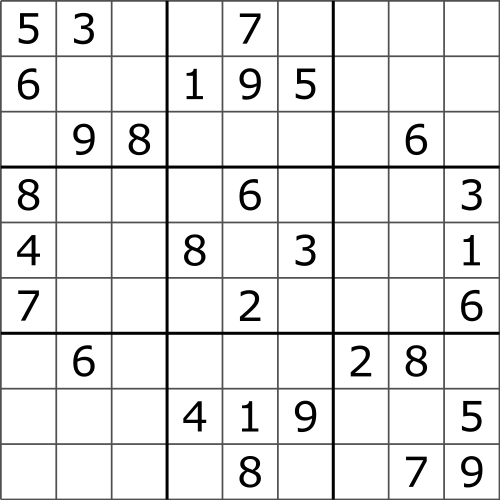
\includegraphics[scale=0.3]{assignment-1/images/sudoku_rules/sudoku-start.png}
    \caption{Starting, partially completed, Sudoku grid}
    \label{fig:sudoku_start}
\end{figure}

\begin{figure}[h]
    \centering
    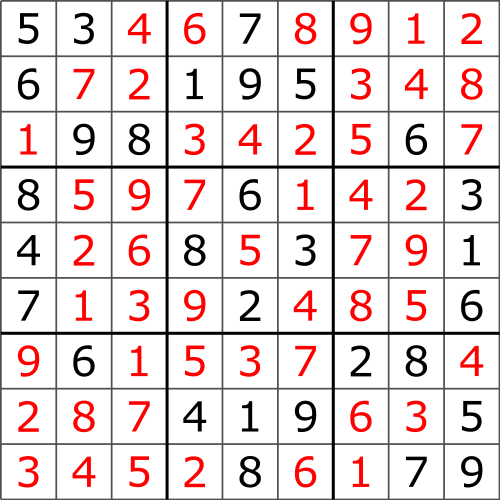
\includegraphics[scale=0.3]{assignment-1/images/sudoku_rules/sudoku-complete.png}
    \caption{Solution to the above presented Sudoku}
    \label{fig:sudoku_complete}
\end{figure}